\chapter[Transcription: Making a Working Copy of DNA]{Transcription: Making\protect\\ a Working Copy of DNA}

\begin{kaichang}
Imagine an heirloom cookbook with a leather cover, yellowed pages, and your great-grandmother's handwritten notes. The family rule is that it must \textbf{never enter the kitchen}: oil, water, and fire could ruin the only copy. But today you are making its braised pork and need one page. What should you do?

You already know: take ordinary notepaper, \textbf{copy the page}, and bring that into the kitchen. Once cooking is done, a dirty note can be discarded. The original remains safe on the shelf, ready to copy again.

Before dismissing this as simple, move the scene into any cell in your body. Its ``heirloom cookbook'' is DNA, a unique complete set so precious that every cell provides a membrane-bound ``safe,'' the nucleus (Chapter 66 explained why its structure suits archiving). Yet the working ``kitchens,'' protein-making ribosomes, all lie \textbf{outside} the nucleus in the cytoplasm. If the cookbook stays in storage but the kitchen is outside, how does copying work? What paper and letters are used, who copies, and what happens to mistakes?

Write down a guess. By the end, the cell's solution will look remarkably like copying a recipe, except its ``scribe'' is a protein machine and its note is RNA.
\end{kaichang}

\section{Moving Information Between Two Rooms}

As usual, observe before explaining.

Biologists in the 1950s had several firm facts. First, staining showed DNA almost entirely in nuclei, hardly ever leaving. Second, protein-making ribosomes were in the cytoplasm, with no DNA nearby during busy protein synthesis. Third, cells contained another similar nucleic acid, RNA (ribonucleic acid), appearing in both nucleus and cytoplasm: \textbf{present at both ends}. Fourth, cells making more protein contained more RNA. Pancreatic cells churning out digestive enzymes and rapidly dividing bacteria had extraordinary RNA amounts, whereas dormant cells making almost no protein had very little.

A further observation was subtler. Scientists briefly let cells ``eat'' radioactive uracil, a raw material particular to RNA (its special feature comes shortly), and followed the radioactivity. Within minutes it appeared first in nuclei, then gradually on cytoplasmic ribosomes. Something seemed to be made in the archive and delivered to the kitchen door.

Combine the clues and a hypothesis emerges. DNA stays inside but must send information to outside ribosomes; RNA visits both places, and its abundance tracks protein production. Perhaps information travels like this: nuclear DNA serves as the master, the cell copies the needed page into RNA, and the copy leaves for a ribosome. This ``portable working copy'' is our subject. Making RNA from DNA is \textbf{transcription}.

\section{RNA: A Lighter Version of DNA}

Zoom to particles. How similar are RNA and DNA, and how do they differ? Chapter 66 described DNA as nucleotides linked into a long chain, each nucleotide comprising phosphate, a five-carbon sugar, and a nitrogenous base. Sugars and phosphates alternate in the backbone; bases project as ``letters.'' RNA has the same basic construction with three consequential changes.

\begin{itemize}[itemsep=2pt]
\item \textbf{The sugar carries an extra oxygen}. DNA contains deoxyribose; RNA contains ribose, with an extra hydroxyl group (\chem{-OH}) on the sugar's second carbon. This extra group is a ``busy character,'' making RNA more vulnerable to chemical attack and enzymatic breakdown. RNA is therefore \textbf{inherently short-lived}.
\item \textbf{U replaces T}. DNA uses A, T, G, C; RNA uses A, U, G, C. U, uracil, closely resembles T, thymine, and still pairs with A. Think of U as a ``simplified T'' without its little methyl tail.
\item \textbf{Usually just one strand}. DNA has two strands wound into a helix; RNA usually works alone. A single strand lacks a protective partner or backup, but can fold freely into varied three-dimensional shapes. This becomes RNA's superpower later.
\end{itemize}

\begin{table}[htbp]
\centering
\begin{tabular}{lll}
\toprule
 & DNA & RNA \\
\midrule
Five-carbon sugar & \shortstack[l]{Deoxyribose\\(one fewer hydroxyl)} & \shortstack[l]{Ribose\\(one extra hydroxyl)} \\
Base letters & A, T, G, C & A, U, G, C \\
Usual strands & \shortstack[l]{Two-stranded\\double helix} & \shortstack[l]{Usually single;\\can fold} \\
Chemical stability & \shortstack[l]{High: long-term\\storage} & \shortstack[l]{Low: short-term\\use} \\
Cellular roles & Master, archive & \shortstack[l]{Working copy,\\tool, component} \\
\bottomrule
\end{tabular}
\end{table}

Look back at the changes: as though coordinated, all point to one purpose. RNA is a \textbf{consumable}. A stable master with complementary backups uses DNA; numerous disposable working copies, made and removed as needed, use short-lived, inexpensive RNA. No cell ``thought up'' this division. Natural selection kept the accounts: fragile long-term storage accumulates fatal errors, while mass-producing temporary copies from costly durable material wastes resources. Stability differences match differences in use.

\section{The Scribe's Instruction Manual}

Now the rules. The copying machine is \textbf{RNA polymerase}. ``Polymerase'' means an enzyme joining small units into a chain (Chapter 49 described enzymes as protein machines changing reaction pathways and lowering activation barriers, not supplying energy). Its manual has five rules.

First, \textbf{do not copy from page one; start wherever a label says to}. Near each gene's beginning lies a special base sequence, the \textbf{promoter}, a ``start copying here'' tag. RNA polymerase slides along DNA, recognizes a promoter, and binds firmly. Transcription is therefore \textbf{selective}: the cell copies only genes for proteins currently needed, not the whole genome. Whole-genome copying belongs to replication (Chapter 67); never confuse the processes.

Second, \textbf{use only one strand as template}. Polymerase locally pries open the helix into a ``transcription bubble'' a dozen or so base pairs across. It reads only one template strand, applying familiar complementarity: template A pairs with U, T with A, G with C, and C with G.

Third, \textbf{copying always runs from $5'$ to $3'$}. Chapter 66 explained DNA's directionality; RNA has it too. The new strand extends only $5'$ to $3'$. As polymerase reads and moves, the opened helix closes behind it, and the growing RNA strand is ``spat out'' of the bubble, trailing ever farther.

Fourth, \textbf{energy comes from the building blocks}. The units are four nucleoside triphosphates (NTPs), ``letters with built-in batteries.'' As each enters the chain, its two-phosphate tail detaches, lowering the system's total energy and driving the reaction forward. The principle matches Chapter 50's ATP: energy belongs to the difference across the whole reaction, not a particular bond. Transcription therefore needs no external energy input; the substrates drive chain growth.

Fifth, \textbf{stop at ``The End.''} A termination signal lies at the gene's end. One common bacterial design is clever: the transcribed sequence folds into a ``hairpin'' followed by a string of U bases. Single-stranded RNA's folding superpower now matters. This structure stalls polymerase and makes it release the RNA, ending transcription.

One often-overlooked but crucial additional rule: \textbf{the same gene can be copied repeatedly}. Bacterial RNA copies often disappear within minutes, but if the protein remains needed, polymerase can return repeatedly to the promoter, producing dozens or hundreds of copies. The master stands firm while copies flow.

\begin{qiaoliang}
How much work does selective copying save? E. coli has about $4.6\times 10^{6}$ base pairs. Even at around 1000 bases per second, full replication (Chapter 67) takes about forty minutes. An ordinary gene's coding region is about 1000 nucleotides, while bacterial RNA polymerase copies 40--80 letters per second: \textbf{one gene takes only about twelve to twenty-five seconds}. Consider the output too: during an mRNA's few-minute bacterial lifetime, ribosomes can repeatedly read it to produce dozens of identical proteins. Twenty seconds to copy a page buys dozens of products. Copy the whole 4.6-million-letter ``book'' every time, and copying alone takes forty minutes while manufacturing millions of currently useless letters. Selectivity is this information system's most valuable rule.
\end{qiaoliang}

\section{Writing the Rules in Symbols}

Only now do symbols appear. Suppose a short DNA template is

\[ \text{DNA template:}\quad \text{3'-TAC GGA CTA-5'} \]

Apply ``A with U, T with A, G with C, C with G, in opposite directions,'' and obtain

\[ \text{Messenger RNA:}\quad \text{5'-AUG CCU GAU-3'} \]

Notice three things: RNA contains no T, with template A giving U; directions oppose (template read $3'$ to $5'$, new strand written $5'$ to $3'$); and this RNA sequence nearly matches DNA's \textbf{other}, non-template strand, except U replaces T. That strand is therefore often called the ``coding strand.''

The following diagram collects the process. As always, circles and lines are human representations; their sizes and shapes are not actual molecular appearances.

\begin{center}
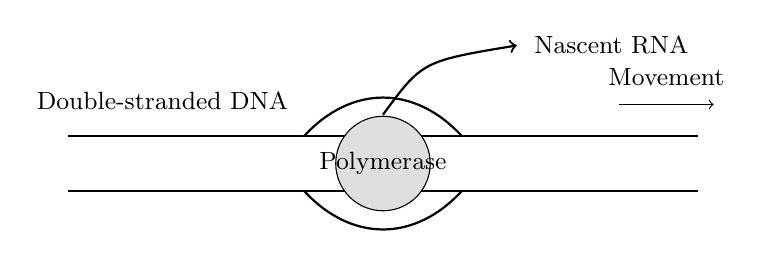
\begin{tikzpicture}[scale=1,every node/.style={font=\small}]
\draw[thick] (0,0.35) -- (8,0.35);
\draw[thick] (0,-0.35) -- (8,-0.35);
\draw[thick] (3,0.35) .. controls (3.6,1.0) and (4.4,1.0) .. (5,0.35);
\draw[thick] (3,-0.35) .. controls (3.6,-1.0) and (4.4,-1.0) .. (5,-0.35);
\draw[fill=gray!25] (4,0) circle (0.6);
\node at (4,0) {Polymerase};
\draw[thick,->] (4,0.62) .. controls (4.5,1.3) .. (5.7,1.5);
\node at (6.9,1.5) {Nascent RNA};
\node at (1.2,0.8) {Double-stranded DNA};
\draw[->] (7.0,0.75) -- (8.2,0.75);
\node at (7.6,1.1) {Movement};
\end{tikzpicture}
\end{center}

Polymerase rides DNA, opens a bubble, and releases growing RNA while the double strand recloses behind it.

\begin{shiyan}
\textbf{Play RNA Polymerase with Paper Strips} (a safe paper-and-pencil game).

Materials: white paper, a pen, scissors, and a ruler.

Steps: (1) Draw a 12-box strip and write a DNA template from $3'$ to $5'$, for example TAC GGA CTA TGC. (2) On another strip, copy complementary RNA from $5'$ to $3'$: write U for A, A for T, C for G, and G for C. (3) Place the strips side by side; check opposite directions and no T in RNA. (4) Deliberately miscopy one box, for example replacing a C with A, and see what happens to the remaining line.

Observations: Why must your reading and writing directions oppose? If you forget to replace T with U, how else does the ``RNA'' differ from DNA? Keep the erroneous strip for Chapter 72's mutations.

Safety: Use scissors carefully. This is only a thinking model. Real polymerase copies dozens of letters per second, without ``staring at the wrong box for ages.''
\end{shiyan}

\section{One Gene, One Enzyme: A Great Simplification}

Having covered transcription, face the chapter's most easily distorted statement.

In 1941, American geneticists Beadle and Tatum irradiated red bread mold spores with X-rays to induce mutations. Some mutant strains lost the ability to synthesize a nutrient; each damaged gene disabled exactly one enzyme in its synthesis pathway. They proposed \textbf{one gene makes one enzyme}. Before the chemical nature of genes was known, this was revolutionary: abstract hereditary factors were linked to concrete protein machines. Life's chemical city finally had a bridge between blueprints and machinery.

Scientific history honestly records successive revisions. First, ``one gene, one polypeptide chain'': proteins such as hemoglobin contain two different chain types made by different genes. Second, some gene products are RNA, not protein. Third, eukaryotic genes can be ``cut'' in different ways to make several proteins (details shortly). Today the relationship resembles a \textbf{many-to-many network}: one gene may yield several products; one protein may assemble products from several genes.

This does not mean Beadle and Tatum were wrong. For their era and their enzymes, one-to-one correspondence was common, and the simplification first made genetics experimentally tractable and calculable. Textbook models work this way: start with a simplification capturing the central issue, establish your footing, then learn the boundaries. The rest of this chapter visits those boundaries.

\section{How the Messenger Was Found}

\begin{zhengju}
By the late 1950s, biology faced a contradiction. Evidence placed protein production on ribosomes, yet ribosomal RNA looked much the same across cells. If ribosomes themselves were the blueprint, how could they make insulin today and hemoglobin tomorrow? Two rival hypotheses emerged: every protein has its own ribosome with a permanently attached blueprint, or ribosomes are general-purpose machines temporarily loaded with a short-lived ``messenger.''

In 1961, Brenner, Jacob, and Meselson settled the issue elegantly. They infected E. coli with T2 phage, the virus from Chapter 65's Hershey--Chase experiment. Infection switched bacterial production to viral proteins. Were these made on \textbf{old} bacterial ribosomes or \textbf{new} viral ribosomes?

They ``weighed'' ribosomes. Bacteria first grew in heavy-isotope medium ($^{15}\mathrm{N}$, $^{13}\mathrm{C}$), making all ribosomes heavy. At infection, they moved to ordinary light medium and received radioactive labels for newly synthesized molecules. Newly made viral ribosomes would be light and radioactive; messenger inserted into existing ribosomes would place radioactivity on heavy ribosomes. The result was clear: newly appearing radioactive viral RNA rode entirely on \textbf{old, heavy} bacterial ribosomes. Not one new ribosome was made.

The conclusion: ribosomes are universal machinery; transient RNA blueprints are what change shifts. That year Jacob and Monod named the molecule \textbf{messenger RNA} (mRNA). Earlier clues existed: Volkin and colleagues had observed rapidly renewed RNA after infection, with base proportions reflecting viral DNA, but nobody then dared declare it the blueprint. Evidence chains often unfold this way: clues first, decisive experimental design later, and the interpretation bold enough to join them last.
\end{zhengju}

\section{The RNA Family: More Than Messengers}

mRNA takes the spotlight, but cellular RNA has many other forms. Roughly divide the work:

\begin{itemize}[itemsep=2pt]
\item \textbf{Messenger RNA (mRNA)}: working blueprints copied from DNA, carrying sequence information for protein manufacture.
\item \textbf{Ribosomal RNA (rRNA)}: the main body of the ribosome. More precisely than ``ribosomes make proteins,'' the active site catalyzing amino-acid bond formation is mainly rRNA; proteins mostly provide supporting structure. Thus \textbf{the central protein-making machine is itself an RNA machine}. This overturned RNA's ``mere notepaper'' image and supports the hypothesis that early RNA served as both archive and tool (Chapter 56).
\item \textbf{Transfer RNA (tRNA)}: small RNA folded into a specific shape, recognizing mRNA letters at one end and holding the matching amino acid at the other. It adapts ``nucleic-acid language'' to ``amino-acid language.'' Its operation and the conversion of four letters into twenty amino acids belong to Chapter 69; for now, remember it exists.
\item \textbf{Regulatory RNA}: a large group making no proteins but controlling ``switches and volume.'' MicroRNAs, for example, are only about twenty letters long and pair with specific mRNAs, preventing translation or hastening destruction, like stamping ``void'' on a note. They are important regulators; Chapter 70 explores how cells decide when and how much to transcribe.
\end{itemize}

See the point? Products transcribed from DNA do not all exist to become proteins. Some RNAs are final products themselves: machines, components, switches. This is already the first crack in ``one gene, one protein.''

\section{Eukaryotic Postproduction}

So far, our stage has mainly been bacterial. With no nucleus, bacterial DNA sits directly in cytoplasm, and a newly transcribed RNA can immediately be read by ribosomes. Translation can even begin halfway through transcription, sharing one production line.

You, me, the garden cat, and the windowsill pothos are eukaryotes, with more elaborate rules. Our DNA stays locked inside nuclei; new RNA needs three ``postproduction'' processes before receiving permission to leave.

\textbf{First, add a cap.} As the new RNA's $5'$ end emerges, a specially modified guanine ``cap'' is attached. It protects against enzymes chewing the front and acts as an identity badge for ribosome recognition. Uncapped RNA is not recognized.

\textbf{Second, add a tail.} The $3'$ end receives a long string of adenines, the poly(A) tail, tens to hundreds of A bases. Like a ``timed fuse,'' it is nibbled by degrading enzymes. Longer tails mean longer mRNA lives and more translations. Different tail lengths change the same mRNA's productive capacity---one hidden regulatory door.

\textbf{Third, and most astonishing, splice.} In 1977, scientists studying a virus infecting human cells found an oddity: its mRNA was \textbf{shorter} than its DNA template and would not align properly. Eukaryotic genes, it turned out, are mostly ``interrupted.'' Useful passages, \textbf{exons}, alternate with stretches absent from final mRNA, \textbf{introns}. Transcription copies everything; a machine called the spliceosome, whose core components are again RNA, removes whole introns and joins exons. The discovery shocked biology, earning Sharp and Roberts the 1993 Nobel Prize.

Splicing's cleverest feature is that \textbf{one initial transcript can yield different final products}. Which exons are retained or skipped can vary: \textbf{alternative splicing}. One gene spliced differently in muscle and nerve cells yields two proteins with different amino-acid sequences and slightly different functions. An extreme example, the fly Dscam gene, can theoretically produce over thirty-eight thousand mRNAs through alternative splicing, more than the fly's total number of genes. Humans have only about twenty thousand protein-coding genes but far more protein types; alternative splicing is an important expansion mechanism.

\begin{wuqu}
``One gene corresponds to one protein.'' This half-century-old statement is a historical simplification, not today's conclusion. Counterexamples abound: (1) Alternative splicing gives fly Dscam tens of thousands of protein versions. (2) Hemoglobin assembles two different polypeptide types from two genes: ``many genes, one protein.'' (3) Many genes produce functional rRNA, tRNA, or microRNA, never becoming protein. More accurately, genes are DNA regions producing functional products, with a many-to-many relationship to proteins. Why do textbooks retain the old phrase? It broadly works in bacteria and many classic cases, making a useful entry model. Treat it as scaffolding, not the building. Chapter 71 will reexamine ``what exactly is a gene?''
\end{wuqu}

\section{The Model's Boundaries}

Every model has limits, and the ``copying model'' demands vigilance in three places.

First, transcription is drawn as one machine moving steadily along a track, but reality is messier: polymerase stalls, backtracks, and is urged on or blocked by other proteins. Promoters vary in strength, and a gene's copying frequency differs enormously across cells and times. A whole regulatory system decides when and how fast to copy in real time---Chapter 70's subject.

Second, ``DNA information flows to RNA, then protein'' holds in most cells, but is no universal iron law. Viruses such as HIV carry reverse transcriptase, which copies DNA from RNA and inserts viral genes into the host genome: the arrow reverses. Influenza and the COVID-19 coronavirus use RNA genomes without involving DNA. The central dogma's arrows show a main route, not a one-way street.

Third, we assumed copies always faithfully match their master. RNA polymerase actually makes roughly one error per ten thousand to a hundred thousand letters, over a hundred times more than DNA polymerase, Chapter 67's proofreading copyist. Transcription lacks replication's stringent proofreading. Why tolerate this? Copies are disposable: one erroneous RNA makes at most one defective protein, then is destroyed within minutes while the master remains safe. A DNA-copying error is an archive accident passed to descendants. Different production lines use different quality standards because errors have different \textbf{costs}. Again, the ledger.

\section{Back to the Recipe}

Now fulfill the opening promise and retell the heirloom-cookbook story.

The book is DNA: precious, unique, too valuable to risk in the kitchen, just as DNA hardly leaves its double-membrane-protected nucleus. Your note is mRNA: copied content on ``budget paper,'' short-lived and disposable. An oil-stained note can be discarded without loss. The ``start here'' tab is a promoter; you, holding the pen, are RNA polymerase; the recipe's ``The End'' is a termination signal.

There are differences. You make one copy at a time; cellular polymerases can queue at one promoter and copy a gene concurrently. Your finished copy works immediately; eukaryotic copies need caps, tails, and splicing, like notes laminated and bound before export. You carry your note into the kitchen and cook yourself; cells hand mRNA to a general-purpose ribosome, whose reading alphabet differs entirely from the cookbook's.

\section{After the Note Arrives}

First, one real application showing how this knowledge changed medicine. You have probably heard of mRNA vaccines. The idea is beautifully direct: since ribosomes recognize mRNA, synthesize a strand encoding a small characteristic viral protein and deliver it into human cells. Ribosomes translate this ``foreign note'' into protein, letting the immune system meet the enemy's appearance in advance and learn recognition (Chapter 61's immune memory). The note degrades quickly, while the virus never entered your body. Every element of this chapter---promoters, caps, tails, RNA's short lifetime---makes the technology possible. Scientists even supply special caps and tails so vaccine mRNA lives long enough and translates sufficiently.

Once the note reaches a ribosome, the real challenge begins. mRNA remains in nucleic-acid language: four letters, A, U, G, C, in a row. The desired protein is a chain of twenty amino-acid types. How can four letters direct twenty components? Are groups of three enough? Who translates? Chapter 69 explores exactly that: translation, turning four letters into twenty amino acids. The blueprint is copied; now read it and build.

\begin{tiaozhan}
Perhaps one question has been bothering you: why does DNA use T while RNA uses U? The difference is tiny, one methyl group. Why distinguish masters from copies? A widely accepted explanation cleverly exploits their long-lived and short-lived roles. Cytosine slowly deaminates spontaneously in water into uracil, a common form of DNA ``paper decay.'' If U were a normal DNA letter, repair enzymes could not tell whether a U belonged or came from damaged C. Choosing T, a ``tagged U,'' makes the rule simple: \textbf{any U in DNA is an accident; replace it}. Cells really have a specialized patrol, uracil glycosylase, finding and removing genomic U daily. Why does RNA not care? It is disposable; one or two errors matter little, so paying an extra methyl group per letter and maintaining recognition machinery is unnecessary. Even alphabet choice reflects the balance between storage cost and error cost.
\end{tiaozhan}

\section*{Try It Yourself}

\begin{sikaoti}
\item Draw information flow from ``the cell needs a protein,'' through DNA, promoter, RNA polymerase, mRNA, and ribosome. Label each arrow with location (inside or outside the nucleus), inputs consumed, and outputs produced.
\item A DNA template reads $\text{3'-ATT GCG TAC-5'}$. Write its mRNA with $5'$ and $3'$ ends, then the other DNA strand, the coding strand. Compare coding DNA and mRNA.
\item Bacterial mRNAs average only minutes of life, human-cell mRNAs hours. Using master-versus-copy roles, explain why short-lived copies can be advantageous. What trouble could a mutation making one mRNA indestructible cause?
\item Replication in Chapter 67 and transcription here both use polymerases but differ greatly. Tabulate template extent (whole genome or local), number of products, proofreading, and error consequences, explaining each difference.
\item Dscam can produce tens of thousands of protein versions without making the fly genome ten thousand times larger. Illustrate alternative splicing of one initial transcript into two products, using boxes for exons and lines for introns.
\item Retroviruses such as HIV copy RNA into DNA. What is wrong with ``hereditary information flows only from DNA to RNA''? How does this inform the idea of the central dogma as a main route rather than an iron law?
\end{sikaoti}
